\chapter{Use cases with Simplified tools}


%-------------------------------------------------------------------
%-------------------------------------------------------------------
%-------------------------------------------------------------------

\section{The Vincennes data set}

%-------------------------------------------------------------------

\subsection{Description of the data set}
\label{Vincennes:DataSet}

On {\tt micmac\_data/ExempleDoc/} the directory {\tt Vincennes} contains
$106$ of the Vincennes's castel \footnote{they are low resolution images
to limit the  downloading time}. This data set illustrate how
the tools described here can be used to achieve a typical architectural task :
compute for each of the main facade an ortho photo, these ortho photo
must be referenced in the same  coordinate system.  Although the ortho-cylindric
option for geometry describe to process thi acquisition seems a very specific
and narrow technicall case, practically it corresponds to very current case
for facade processing.


The $106$ of Vincenne's data set are organized in $4$ subset :


\begin{itemize}
   \item  images {\tt Face1.*} correspond to the first facade;
   \item  images {\tt Face2.*} correspond to the second facade;
   \item  images {\tt  Lnk12.*} images acquired to make the link between
           the two facades;
   \item  images {\tt  Calib.*} acquired to have easily a first
           calibration.
\end{itemize}

Note that, \emph{before any processing}, the images have been renamed taking 
into account the acquisition structire. It is highly recommanded to do the
same thing before processing  set of data having some complexity. It avoid
the creation of tricky regular expression. These image are jpeg low resolution
images to limit the bandwith when one upload the data, but of course in
real case the full resolution raw image will be prefered.


\begin{figure}
\begin{center}
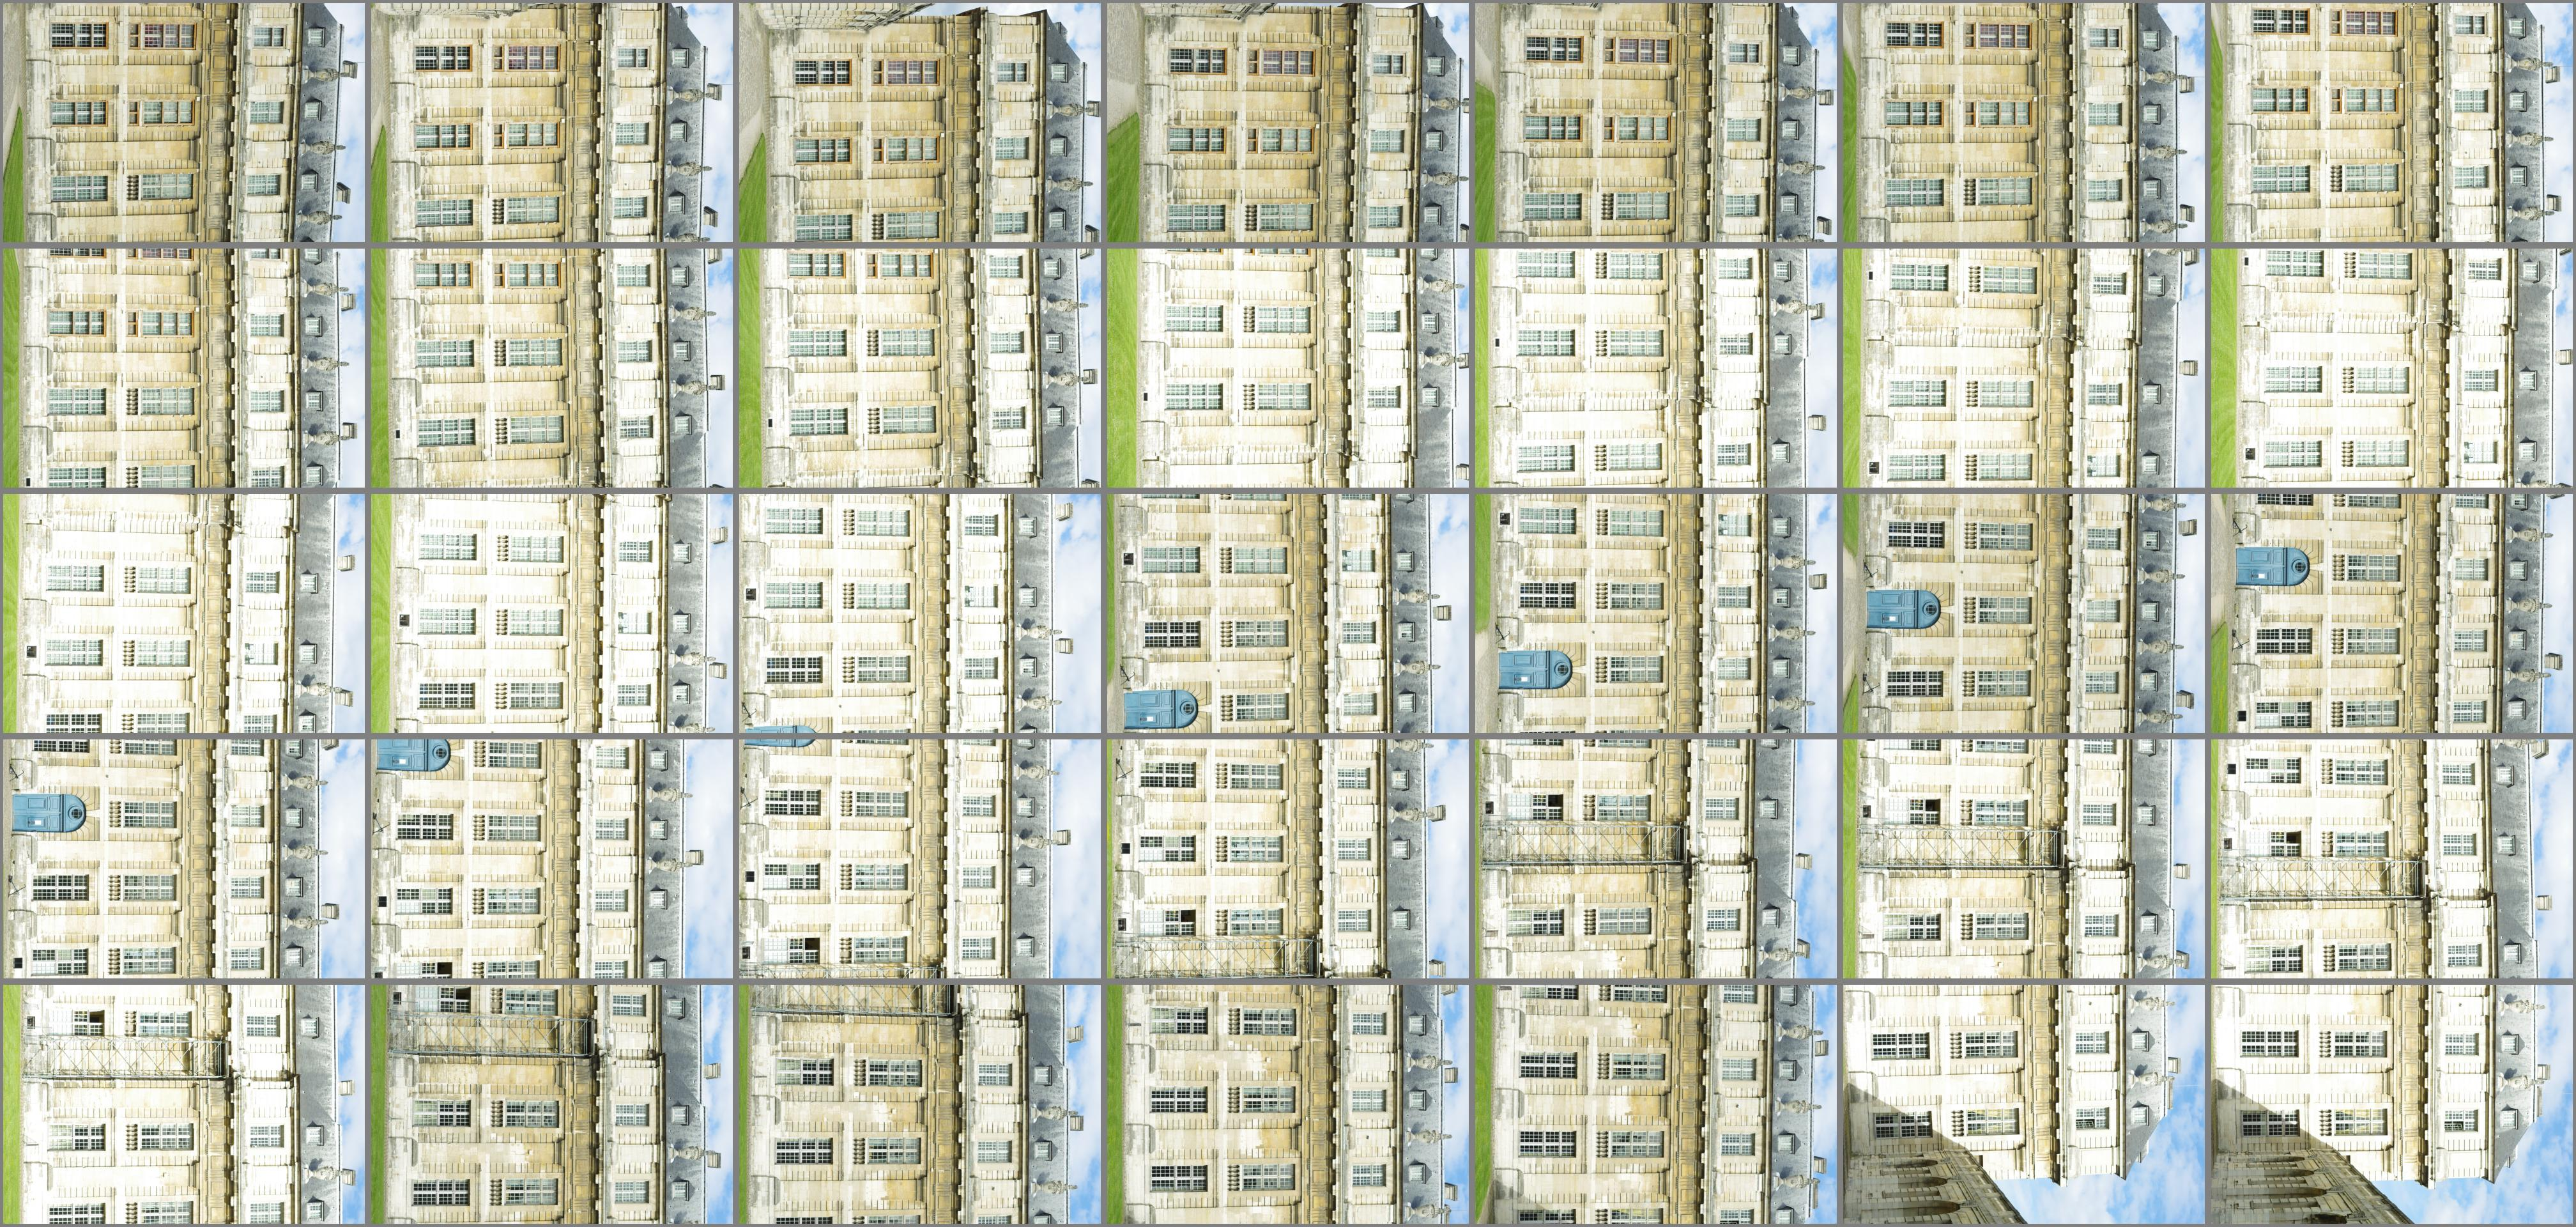
\includegraphics[width=120mm]{FIGS/Vincennes/Planche-F1.jpg}

\vspace{0.3cm}
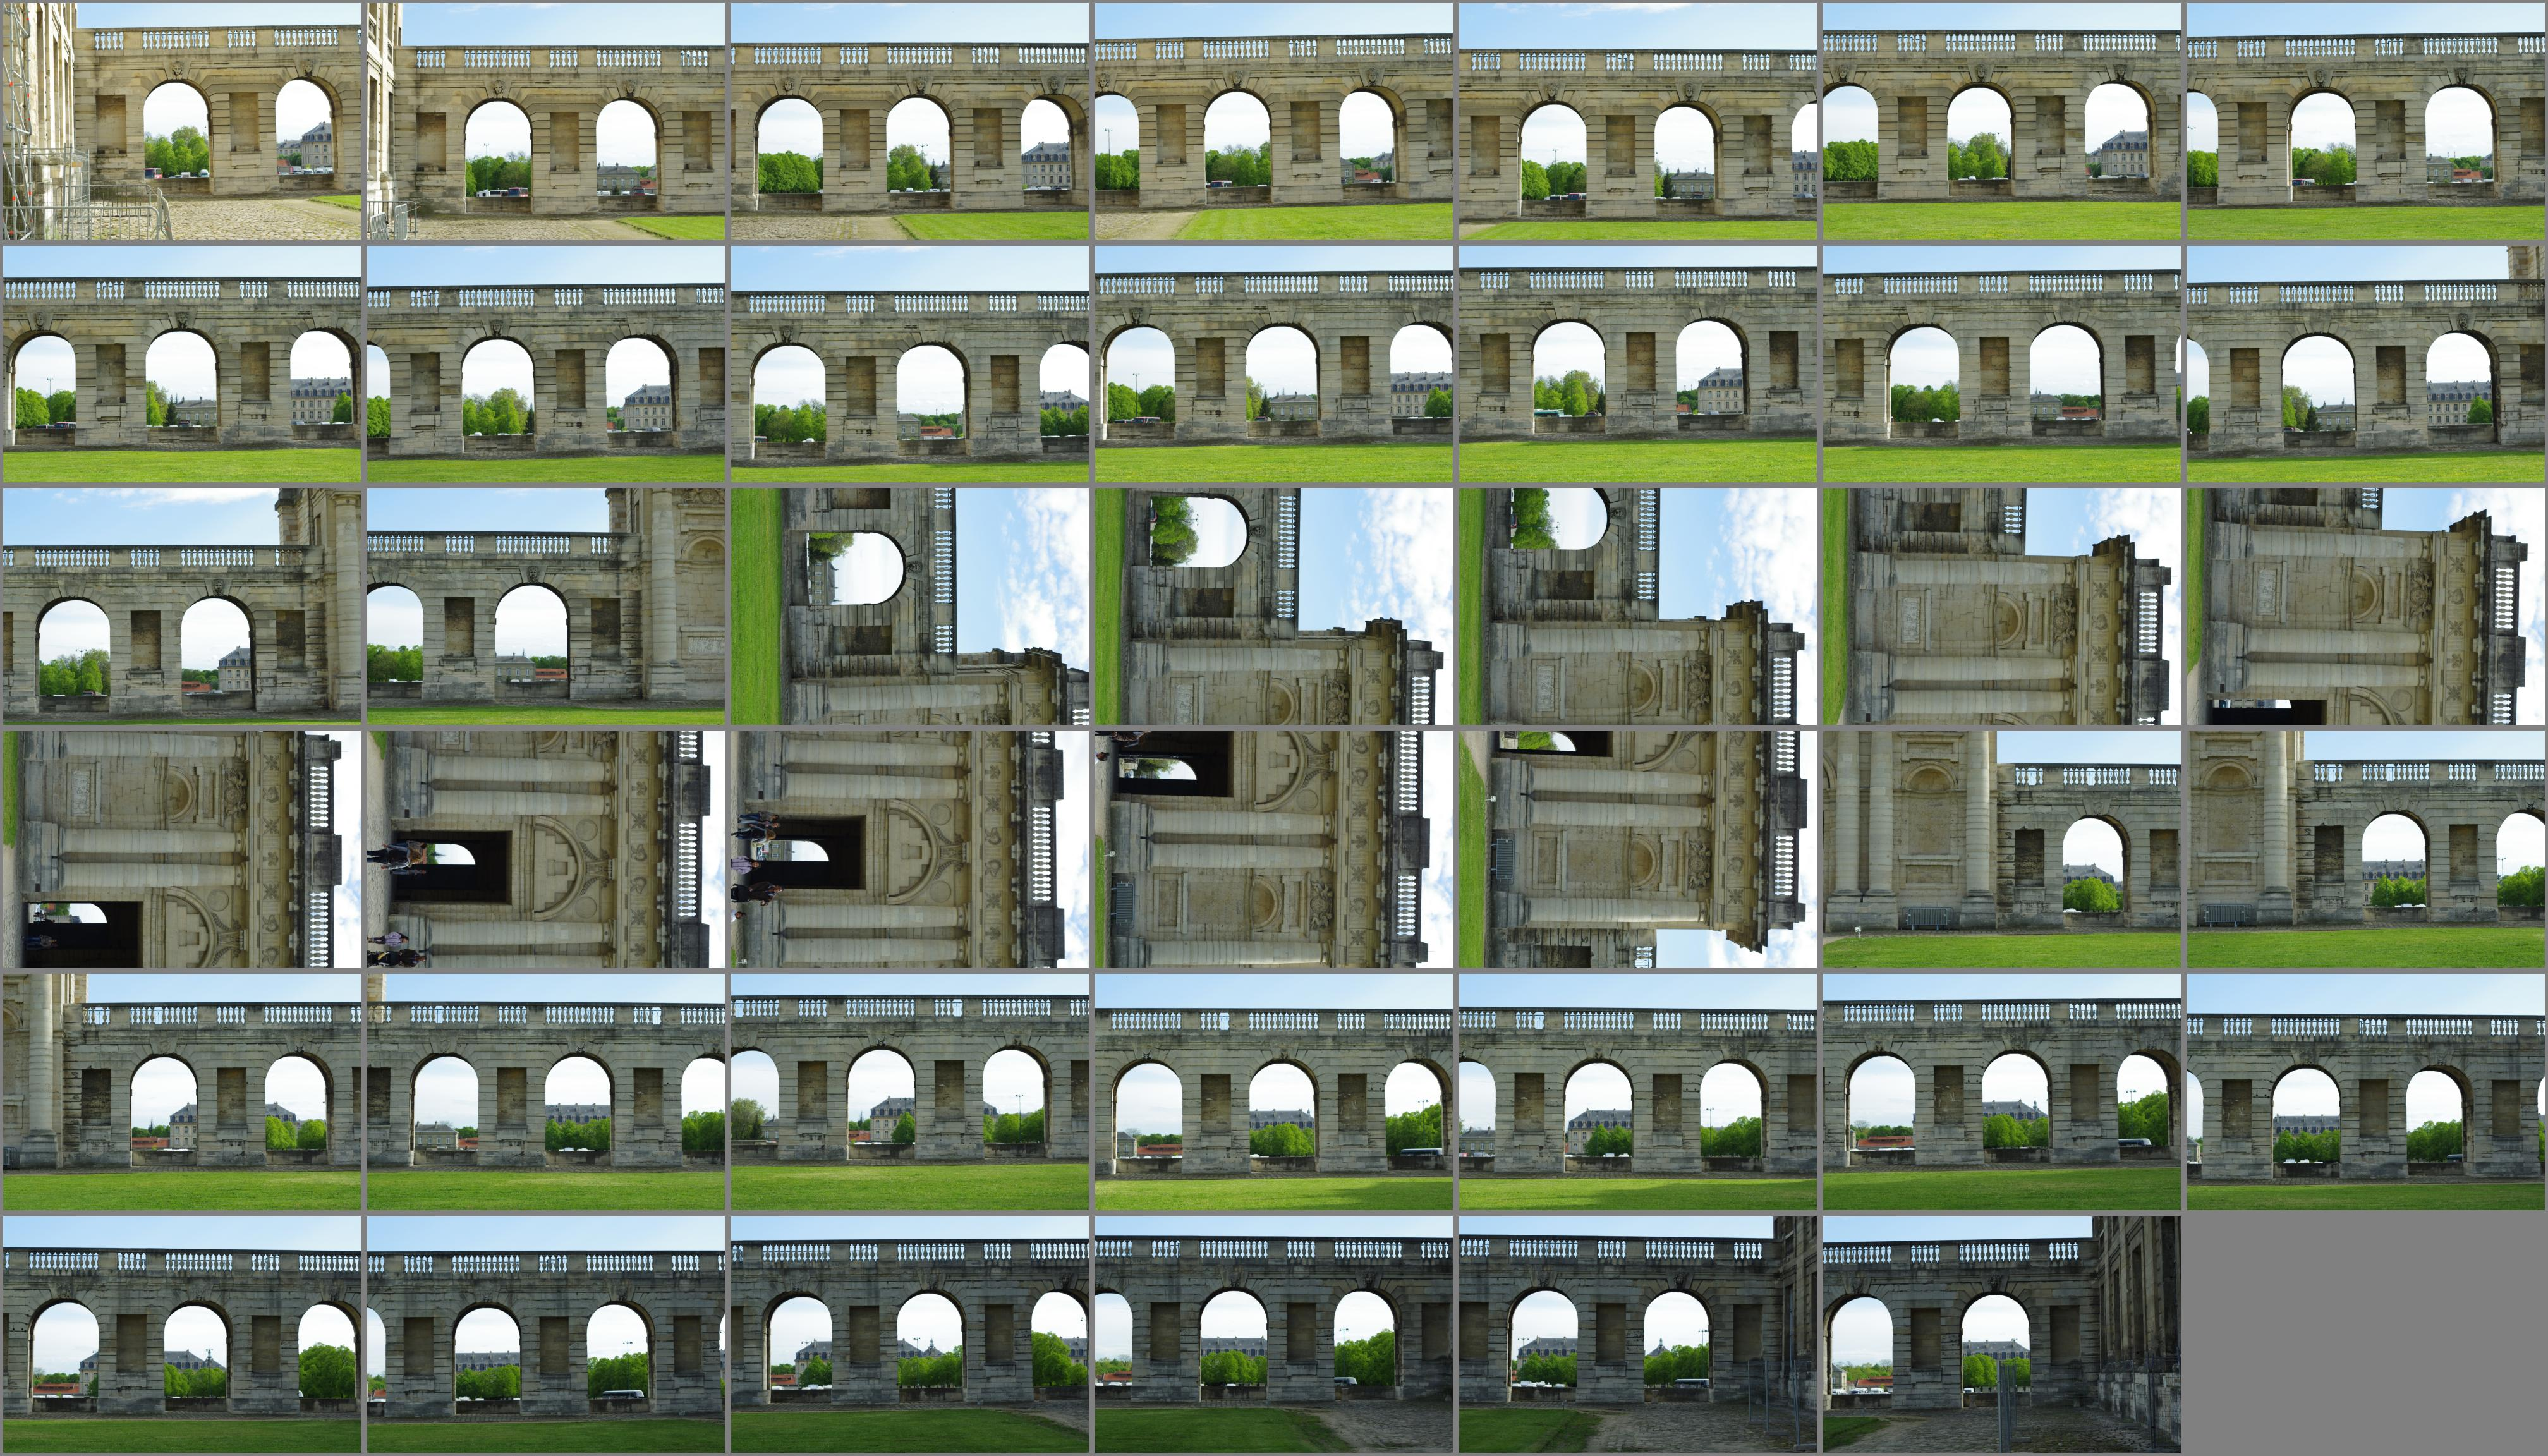
\includegraphics[width=120mm]{FIGS/Vincennes/Planche-F2.jpg}

\vspace{0.3cm}
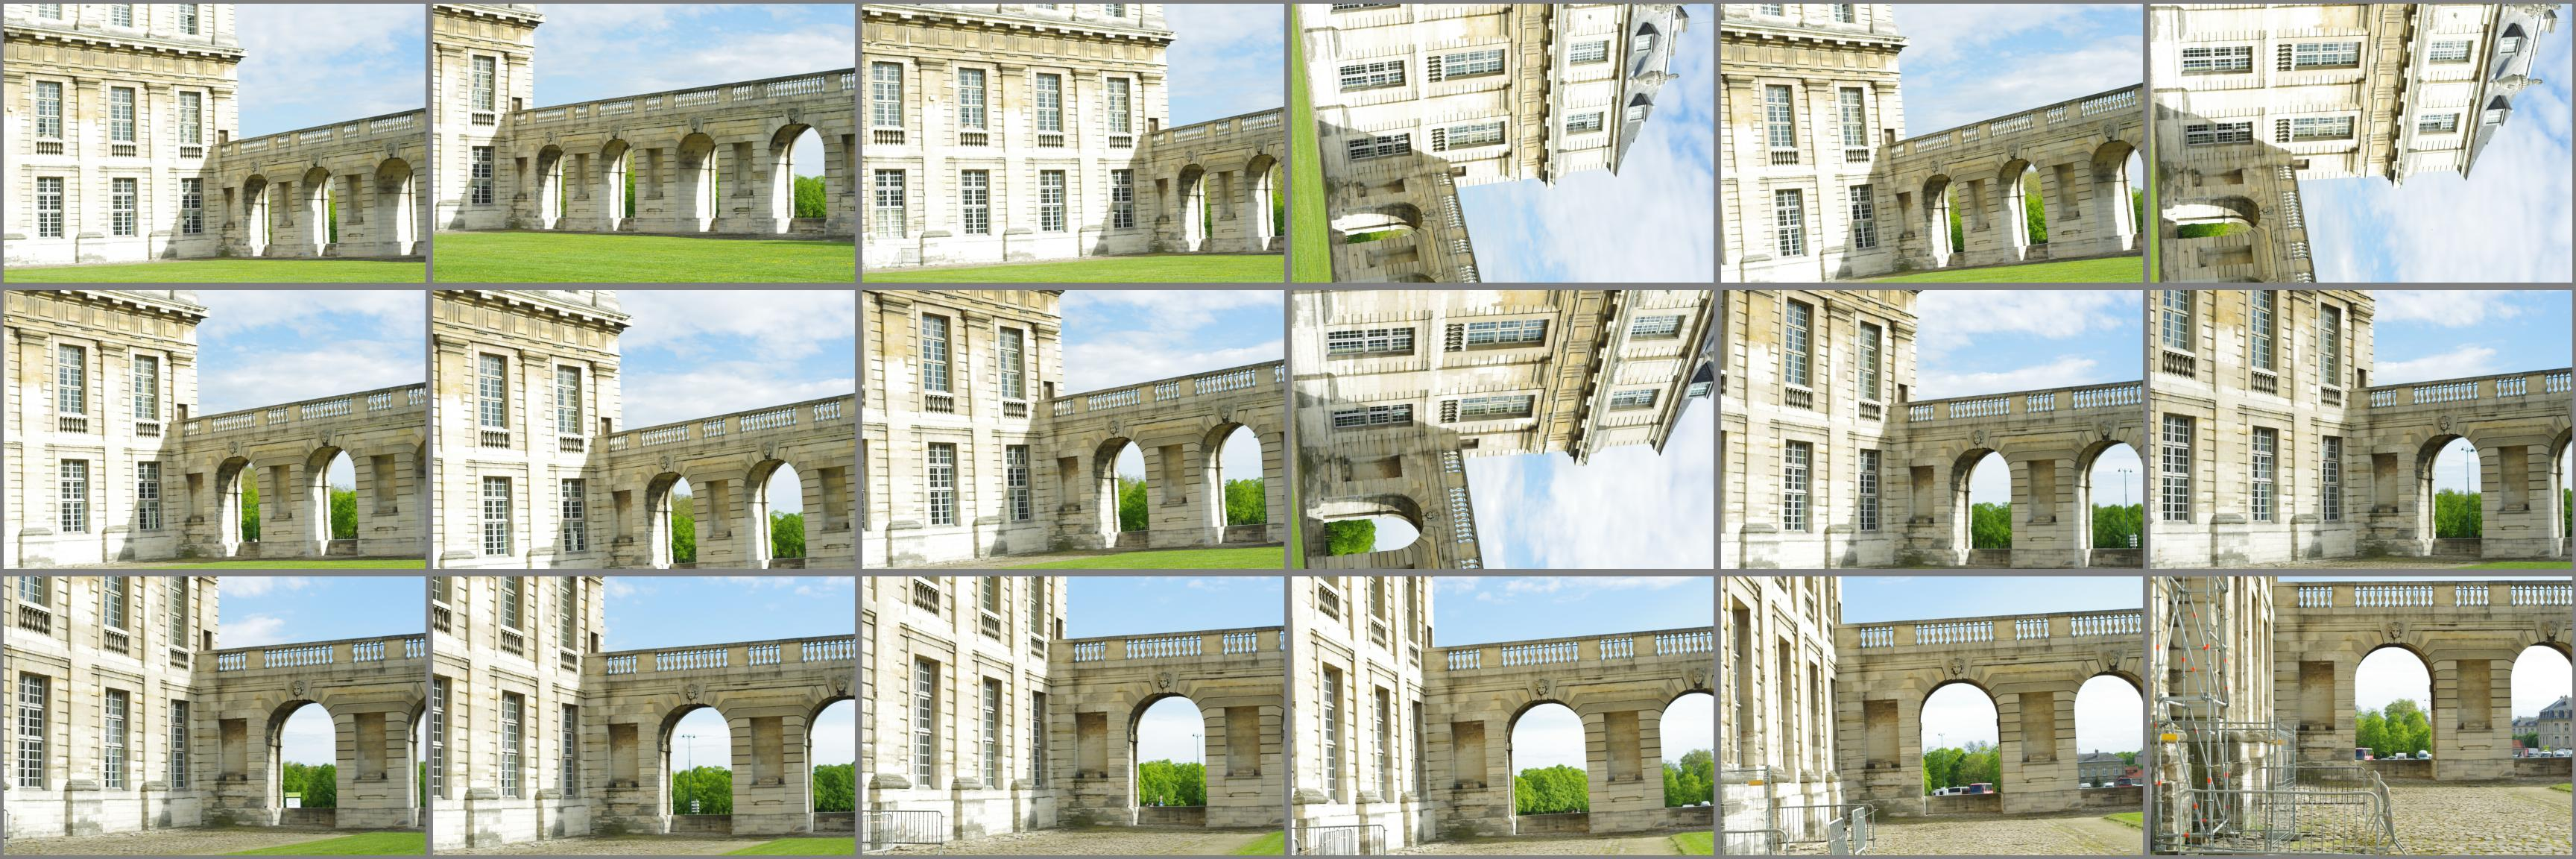
\includegraphics[width=120mm]{FIGS/Vincennes/Planche-Lnk.jpg}

\vspace{0.3cm}
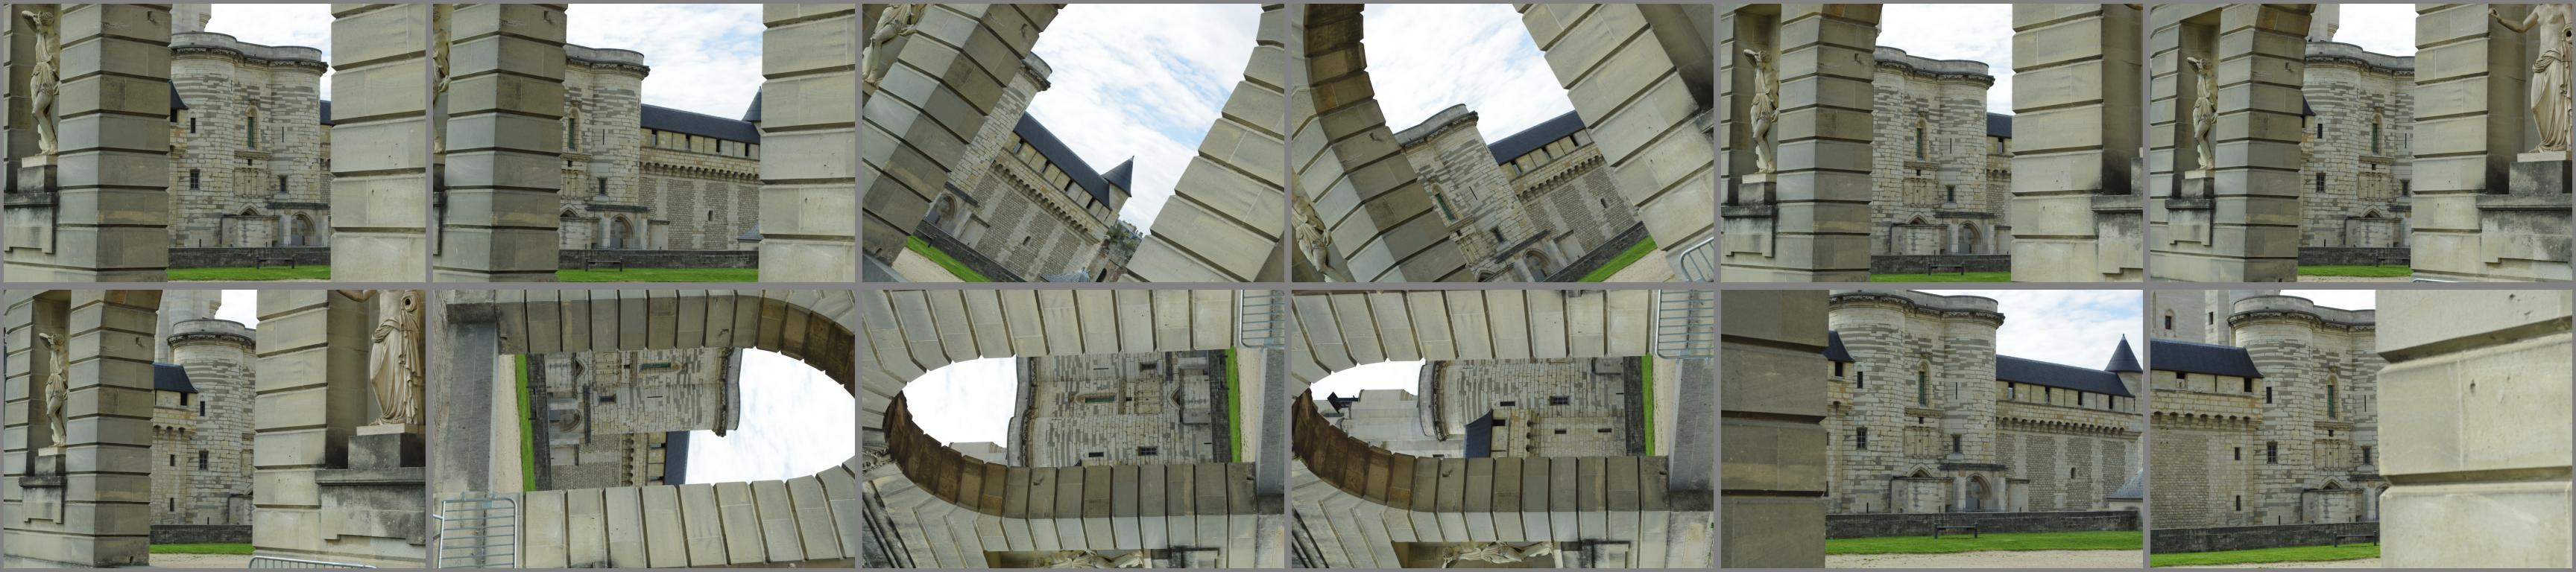
\includegraphics[width=120mm]{FIGS/Vincennes/Planche-Calib.jpg}
\end{center}
\caption{Image of Vincenne's data set : Face1, Face2, Lnk12 and Calib }
\label{FIG:Glob:Vincenne}
\end{figure}




The file {\tt  ExeCmd.txt} contains all the command that will entered.


%-------------------------------------------------------------------

\subsection{Computing tie points and orientations}

    %  -  -  -  -  -  -  -  -  -  -  -  -

\subsubsection{Tie points}

The computation of tie points and relative orientation is quite
classic now. 

For tie points we want to compute:

\begin{itemize}
   \item  points  between all pairs of calibration data set;
   \item  points  of \emph{Face1} and \emph{Face2} using the linear structure of
          the aqcuisition;
   \item  points  between \emph{Lnk12} and connected subset of  \emph{Face1} and \emph{Face2};
\end{itemize}

This is done by :

\begin{verbatim}
Tapioca All  "Calib-IMGP[0-9]{4}.JPG" 1000
Tapioca Line "Face1-IMGP[0-9]{4}.JPG" 1000 5
Tapioca Line "Face2-IMGP[0-9]{4}.JPG" 1000 5
Tapioca All  "((Lnk12-IMGP[0-9]{4})|(Face1-IMGP529[0-9])|(Face2-IMGP531[0-9])).JPG" 1000
\end{verbatim}

    %  -  -  -  -  -  -  -  -  -  -  -  -

\subsubsection{Relative orientaion}

Then we want to make a first calibration with the calibration data set, and
use this calibration as an initial value to the global orientation of
\emph{Face1},  \emph{Face2} and \emph{Lnk12}. This is done by :

\begin{verbatim}
Tapas RadialStd "Calib-IMGP[0-9]{4}.JPG" Out=Calib
Tapas RadialStd "(Face1|Face2|Lnk12)-IMGP[0-9]{4}.JPG" Out=All InCal=Calib
\end{verbatim}

    %  -  -  -  -  -  -  -  -  -  -  -  -

\subsubsection{Option, absolute orientaion}

Finally, we want to transform the orientation from an arbitrary relative 
orientation to some physically based orientation. If we have some ground
control points, this can be done using the {\tt GCPBascule} command (see~\ref{Sec:GCPBascule}) . To
generate orientation in {\tt Ori-Ground} :

\begin{verbatim}
GCPBascule  "(Face1|Face2|Lnk12)-IMGP[0-9]{4}.JPG" All Ground Mesure-TestApInit-3D.xml\
 Mesure-TestApInit.xml
\end{verbatim}

    %  -  -  -  -  -  -  -  -  -  -  -  -

\subsubsection{Option, scene-based orientaion}

Alternatively, if we do not have any GCP and want to put the data in an orientation
having some physical meaning, we can use the {\tt SBGlobBascule} command (see~\ref{ScBas:Basc}) :

\begin{verbatim}
SBGlobBascule "(Face1|Face2|Lnk12)-IMGP[0-9]{4}.JPG" All MesureBascFace1.xml  Glob \
    PostPlan=_MasqPlanFace1  DistFS=2.0 Rep=ij
\end{verbatim}

There is a new option {\tt Rep=ij}, the meaning of this option is :
\label{SGB:Rep}

\begin{itemize}
   \item it is a string that describe a repair;
   \item it must contain $2$ symbols, each symbols can be in \emph{\{i,-i,j,-j,k,-k\}} and desribe a vector;
   \item the globlal orientation with be such that in the final orientation the line 
         defined by {\tt Line1-Line2} is aligned on first vector, and the normal to the plane is aligned on second vector;
   \item here in final orientation $i$ will be the horizontal of the wall and $j$ will be the
         normal to the wall, consequently $k=i\wedge j$ will be the vertical;
\end{itemize}


%-------------------------------------------------------------------
\subsection{Matching}


    %  -  -  -  -  -  -  -  -  -  -  -  -
\subsubsection{"Standard" option}

The "standard pipeline" for generating an ortho photo of facade, 
as seen in~\ref{Simp:Tool:One}, is for each facade :

\begin{itemize} 
   \item compute a local repair to define the facade with {\tt RepLocBascule};
   \item compute a rectified image {\tt Tarama}; 
   \item make the matching with {\tt Malt};
   \item generate the ortho image with {\tt  Tawny};
\end{itemize} 

This can be done by the succession of commands :

\begin{verbatim}
RepLocBascule  "(Face1)-IMGP[0-9]{4}.JPG" Ground  MesureBascFace1.xml Repere-F1.xml\
       PostPlan=_MasqPlanFace1
Tarama  "(Face1)-IMGP[0-9]{4}.JPG" Ground  Repere=Repere-F1.xml  Out=TA-F1 Zoom=4
Malt Ortho  "(Face1)-IMGP[0-9]{4}.JPG"  Ground  Repere=Repere-F1.xml  \
                     SzW=1 ZoomF=1  DirMEC=Malt-F1 DirTA=TA-F1
Tawny Ortho-Malt-F1/
\end{verbatim}

The results are quite deceiving !!! Figure~\ref{FIG:Pb:Vincenne} illustrate the
encountered problem :

\begin{itemize}
    \item on firt line, the ortho photo; it suffer several problem; the main problem
         are located on the roof (due to bad incidence angles) and on horizontal lines;

    \item on second line, a snapshot from Meshlab, showing the camera position;
          it illustrates the fact that in this acquisition all the camera centers are 
         located on the same line;

    \item the third line, focus on the matching problem  that occurs on linear detail that
          are parallel to the line of acquisition; 
\end{itemize}


\begin{figure}
\begin{center}
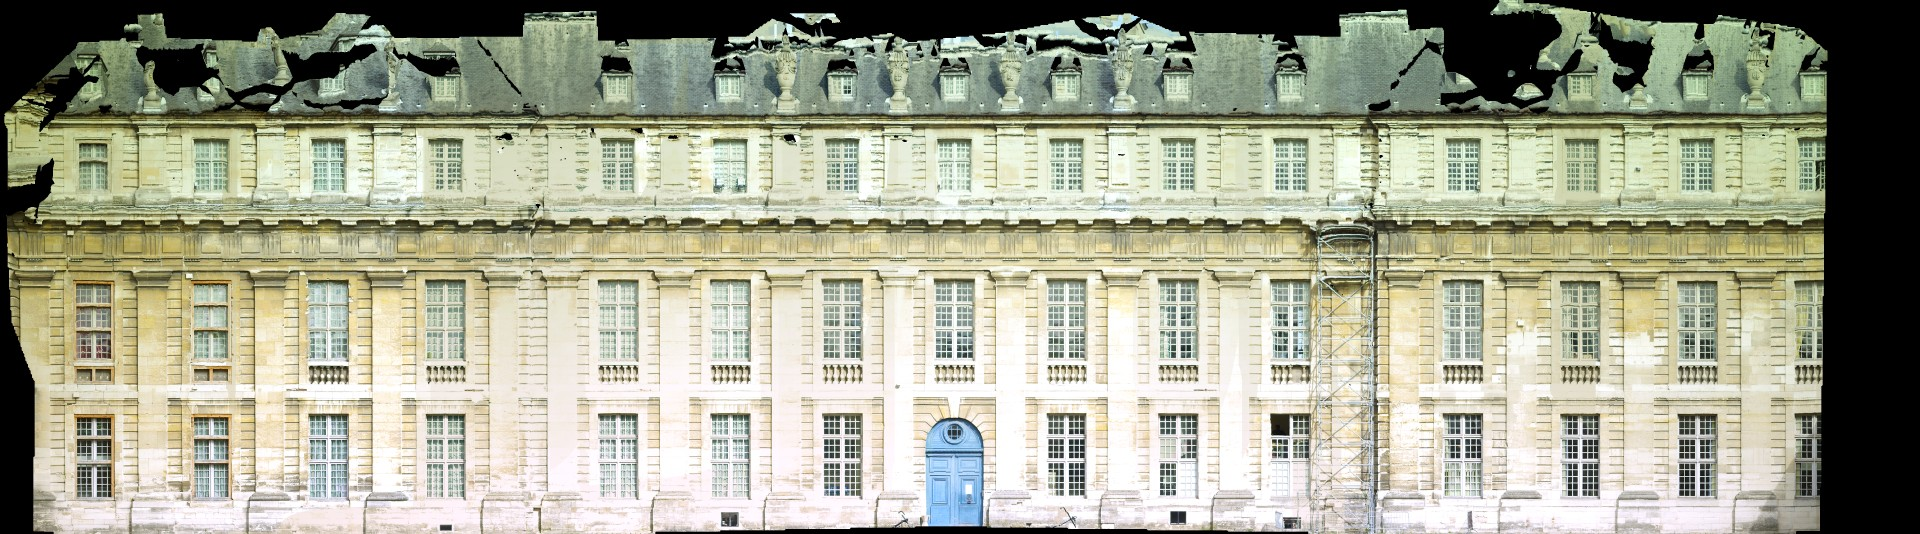
\includegraphics[width=160mm]{FIGS/Vincennes/Ortho-Moche.jpg}

\vspace{0.3cm}
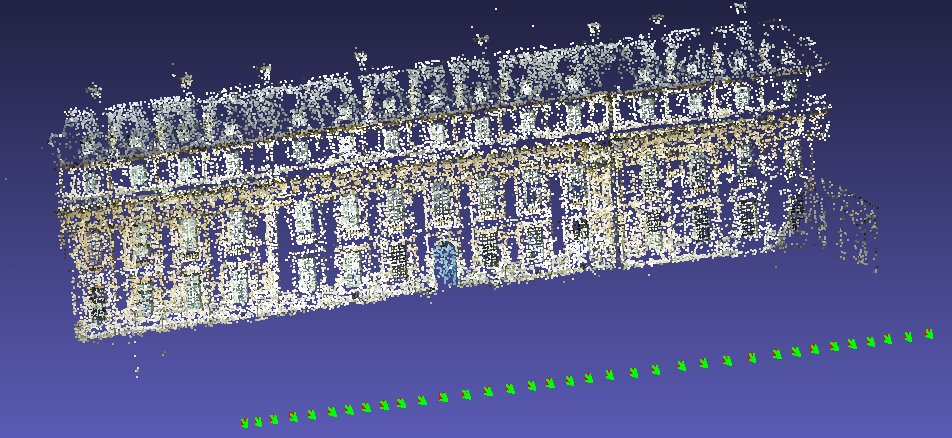
\includegraphics[width=160mm]{FIGS/Vincennes/CamFace1.jpg}

\vspace{0.3cm}
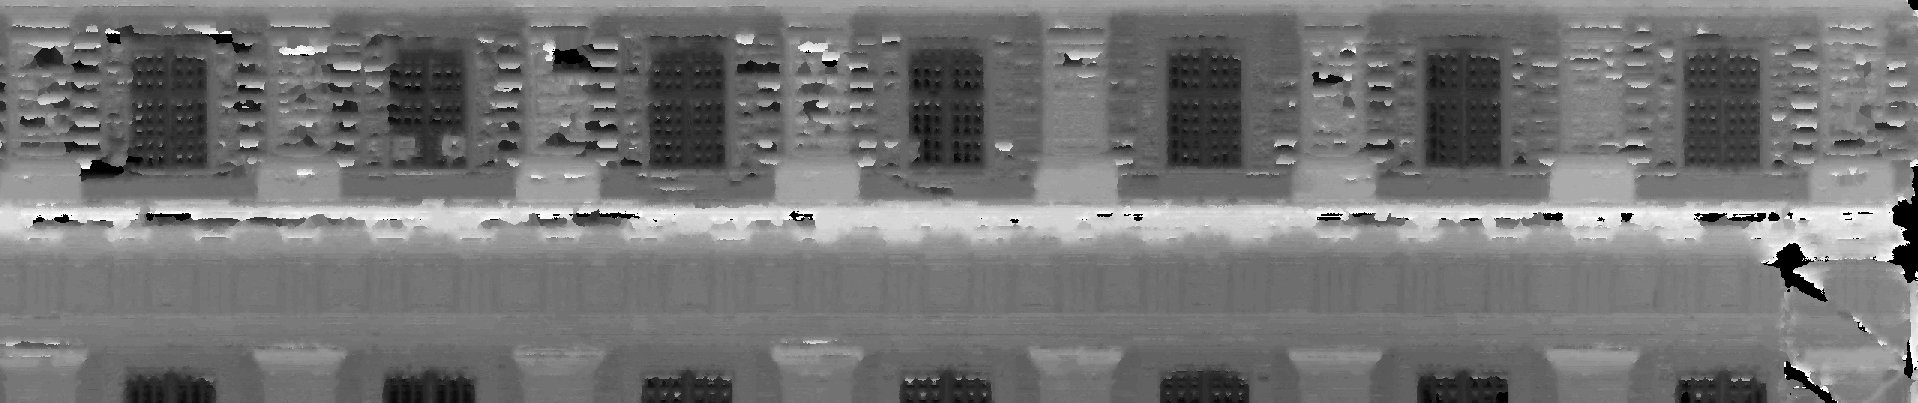
\includegraphics[width=160mm]{FIGS/Vincennes/MNT-Moche.jpg}

\end{center}
\caption{Problem with standard processing on Vincennes Facade : bas quality ortho photo,
aligment of cameras, poor dept map especially for linear structure parallel to camera alignment}
\label{FIG:Pb:Vincenne}
\end{figure}


    %  -  -  -  -  -  -  -  -  -  -  -  -
\subsubsection{"Ortho-cylindric" option}

Intutively it  is obvious that when the camera center are all aligned on the same line,
the matching problem is  ambiguous for line parallel to the acquisition, consequently
the quality of result is poor. 
Obviously, the default would decrease (in fact disappear) if the camera were not
aligned, using an UAV or a scaffolding , we could have an optimal geometry similar
to aerial acquisition. But it is not always possible to have such material and, for economical reason, 
it would be interesting to be abble to obtain a relatively good quality ortho photo even when
all the camera are aligned.

In fact for theoreticall reasons described in~\cite{Penard},
this problem are  much more important in ground geometry than in image geometry.
With the option we have seen until now, we bascically this alternative :

\begin{itemize}
   \item  use the ground geometry with a simple process but obtain bad qualitiy results such those of 
          figure~\ref{FIG:Pb:Vincenne};

   \item  use the image geometry with  good results but have a complicated workflow with many depth map
          that must be merged.
\end{itemize}


With such acquisition, the ortho-cylindrical geometry combine the benefit of these
two geometry. Intuitively this geometry is equivalent to the geometry a virtual push-broom
camera, the line of this virtual push-broom being the line on which are located the 
camera center. More formally :


\begin{itemize}
   \item  let  $X,Y,Z$ be a coordinate system such that $Y=0$ be approximatively line on wich the camera
          are located, and $Z=D$ be approximatvely the plane of the wall;

   \item  let  $U,V,L$ be the coordinate system befined by
\begin{itemize}
    \item  $U= D \tan^{-1} (\frac{X}{Z})$
    \item  $V=Y$ and $L=Z$;
\end{itemize}
   \item   we  will then compute the DSM as a function $L= F(U,V)$.
\end{itemize}

To use this geometry, we just need  to set {\tt OrthoCyl=true} in the command {\tt RepLocBascule} :

\begin{verbatim}
RepLocBascule  "(Face1)-IMGP[0-9]{4}.JPG" Ground  MesureBascFace1.xml Ortho-Cyl1.xml\
   PostPlan=_MasqPlanFace1 OrthoCyl=true
\end{verbatim}

With this option, {\tt RepLocBascule} will also compute, using least meanst square,
the line that fit the best the alignment of camera perspective centers. If we take 
a look at file {\tt Ortho-Cyl1.xml} we can see  this line coded by {\tt <P0>}
and {\tt <P1>}  (plus the previous local repair  {\tt <Repere>}) :

\begin{verbatim}
<XmlModeleSurfaceComplexe>
     <XmlOneSurfaceAnalytique>
          <XmlDescriptionAnalytique>
               <OrthoCyl>
                    <Repere>
                         <Ori>-0.00573  -2.7113574  -0.4521156 </Ori>
                         <Ox>  0.00029   0.9999998  -0.0003715 </Ox>
                         <Oy> -0.00043   0.0003716   0.9999998 </Oy>
                         <Oz>  0.99999  -0.0002960   0.0004372 </Oz>
                    </Repere>
                    <P0>30.392821 -2.720358 -0.438823</P0>
                    <P1>30.391561 -1.720359 -0.43974</P1>
                    <AngulCorr>true</AngulCorr>
               </OrthoCyl>
          </XmlDescriptionAnalytique>
          <Id>TheSurf</Id>
          <VueDeLExterieur>true</VueDeLExterieur>
     </XmlOneSurfaceAnalytique>
</XmlModeleSurfaceComplexe>
\end{verbatim}

    %  -  -  -  -  -  -  -  -  -  -  -  -
\subsubsection{Concrete use of "Ortho-cylindric" option}

It is then sufficient to give the file created by  {\tt RepLocBascule} 
as an optionnal parameter to {\tt Tarama} and {\tt Malt} to compute 
in the adequate geometry; for facade one, we can enter :


\begin{verbatim}
RepLocBascule  "(Face1)-IMGP[0-9]{4}.JPG" Ground  MesureBascFace1.xml Ortho-Cyl1.xml \
        PostPlan=_MasqPlanFace1 OrthoCyl=true
Tarama  "(Face1)-IMGP[0-9]{4}.JPG" Ground  Repere=Ortho-Cyl1.xml  Out=TA-OC-F1 Zoom=4
Malt Ortho  "(Face1)-IMGP[0-9]{4}.JPG"  Ground  Repere=Ortho-Cyl1.xml  \
                   SzW=1 ZoomF=1  DirMEC=Malt-OC-F1 DirTA=TA-OC-F1
Tawny Ortho-UnAnam-Malt-OC-F1/
\end{verbatim}

And for facade 2 :

\begin{verbatim}
RepLocBascule  "(Face2)-IMGP[0-9]{4}.JPG" Ground  MesureBascFace2.xml Ortho-Cyl2.xml \
     PostPlan=_MasqPlanFace2 OrthoCyl=true
Tarama  "(Face2)-IMGP[0-9]{4}.JPG" Ground  Repere=Ortho-Cyl2.xml  Out=TA-OC-F2 Zoom=4
Malt Ortho  "(Face2)-IMGP[0-9]{4}.JPG"  Ground  Repere=Ortho-Cyl2.xml  SzW=1 ZoomF=1  \
          DirMEC=Malt-OC-F2 DirTA=TA-OC-F2 NbVI=2
Tawny Ortho-UnAnam-Malt-OC-F2/
\end{verbatim}

Note some options of these commands :

\begin{itemize}
   \item in {\tt RepLocBascule}, the {\tt OrthoCyl=true} as described above;
   \item in {\tt Tarama}, the {\tt Out=TA-OC-F1} (and {\tt Out=TA-OC-F2}) to specify the
         directory of output; this is naturally to avoid that each call to {\tt Tarama} overwrite
         the result of previous calls;
   \item in {\tt Malt}, the {\tt DirTA=TA-OC-F1} to get the adequete entry from  {\tt Tarama} 
         and {\tt Out=DirMEC=Malt-OC-F1} to specify the results; this change the place are written
         the results of matching, and also the result of individual ortho photo (here it will be 
         {\tt Ortho-UnAnam-Malt-OC-F1/});
\end{itemize}


If the ortho-cylindric geometry is "optimal" for computation, this is 
generally not a proper geometry for the final user , so at the end of the process,
{\tt MicMac} generate an "un-anamorphosed" version of this depth map in
euclidean geometry.  For example on directory {\tt Malt-OC-F1/}, there
exists $9$ files {\tt Z\_NumX\_DeZoomY\_STD-MALT.tif} corresponding to
the different level of matching in ortho-cylindrical geometry, 
and a single file {\tt Z\_Num1\_DeZoom1\_Malt-Ortho-UnAnam.tif}
corresponding to the eulidean version of the last file
( this is the version presented on second line of
figure~\ref{FIG:OK:Vincenne}).
Note that in general there will be very few hidden part on 
ortho-cylindrical depth map; conversely, they are quite current on
euclidean version, but it is intrinsic to what we want to restituate
with such acquisition.
By default, the ortho photo are also generated in euclidean geometry
using the unanamorphosed depth-map. Here for example, they are
generated under {\tt Ortho-UnAnam-Malt-OC-F1/} and {\tt Ortho-UnAnam-Malt-OC-F2/}.


Figure~\ref{FIG:OK:Vincenne} present some results obtained after this process :

\begin{itemize}
    \item first line present the depth-map computed in ortho-cylindric geometry using
           color code;
    \item  second line, euclidean version of the depth map, remark the hidden part;

    \item  third line, ortho photo of facade.
\end{itemize}

\begin{figure}
\begin{center}
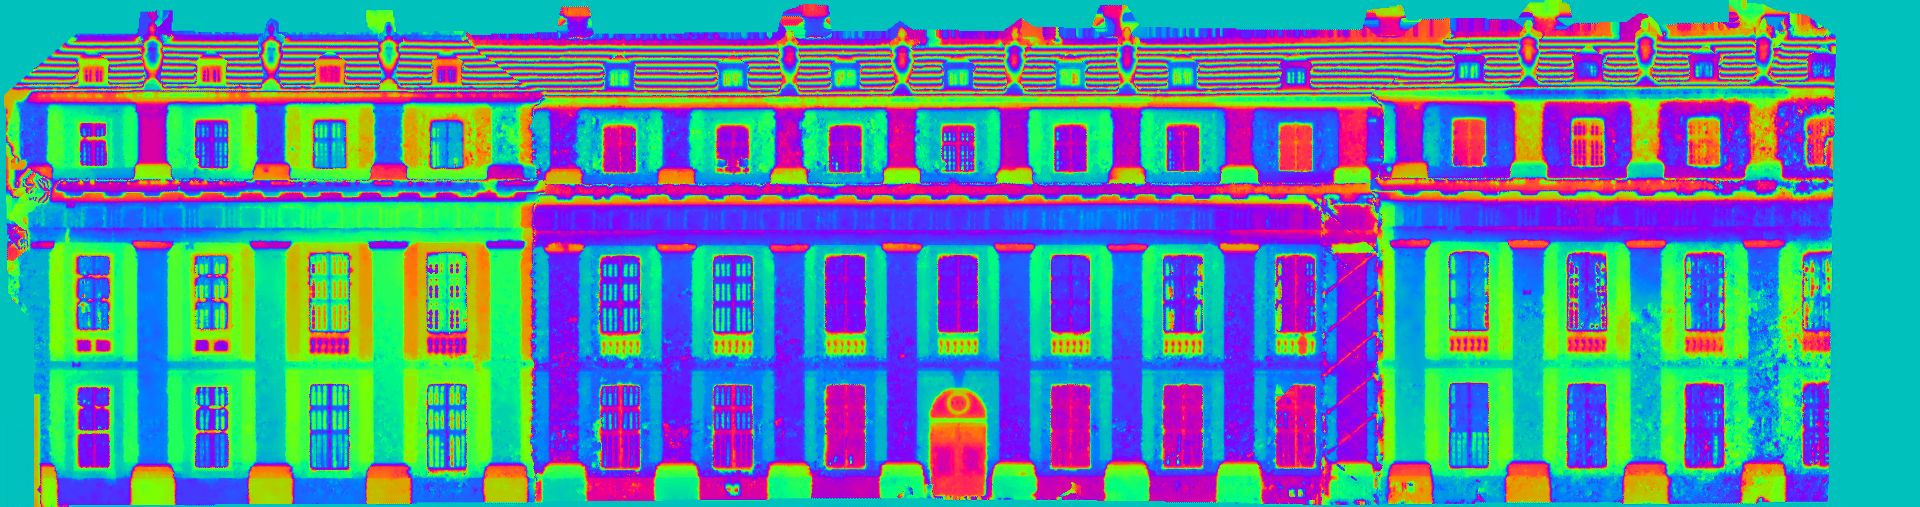
\includegraphics[width=160mm]{FIGS/Vincennes/MNE-OC.jpg}

\vspace{0.3cm}
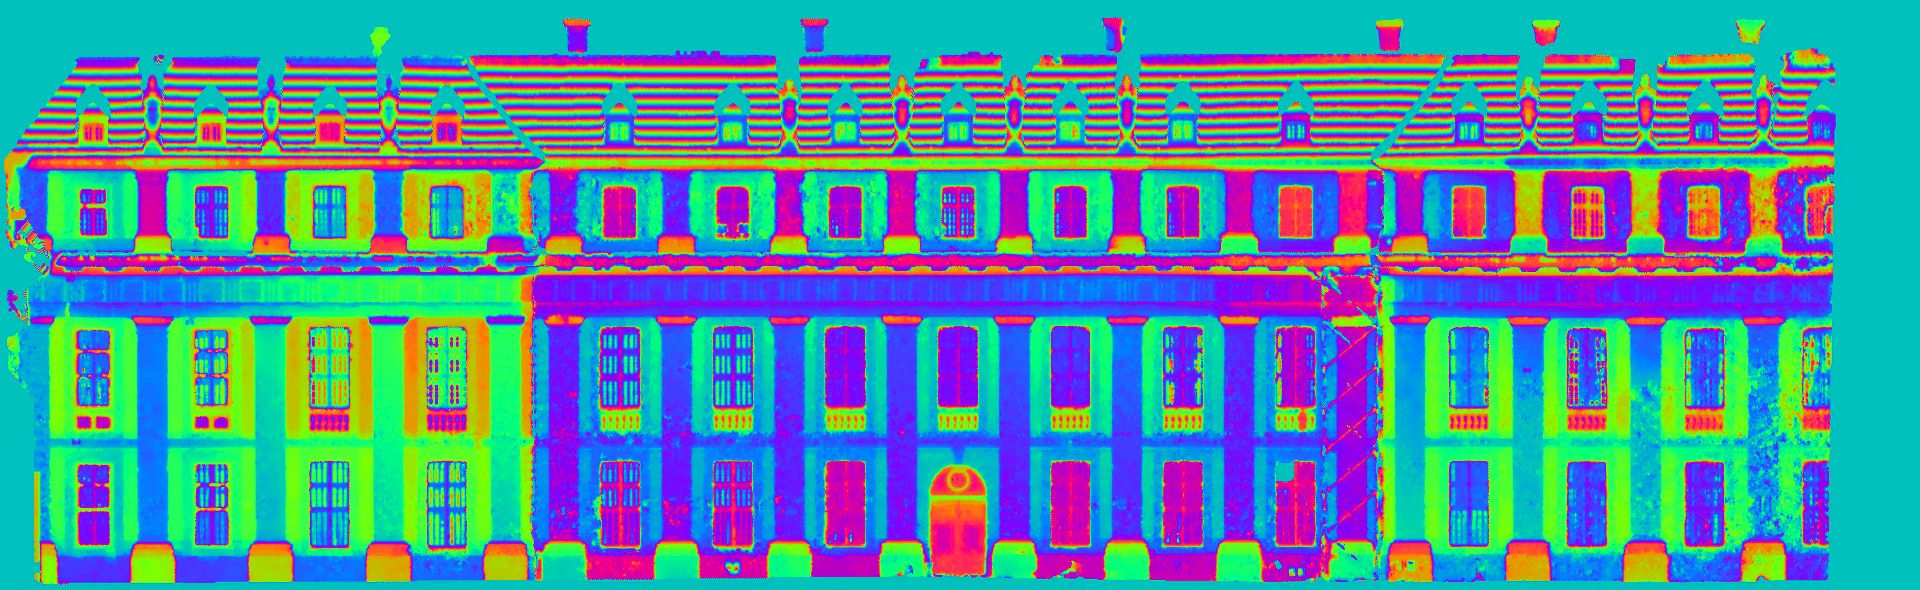
\includegraphics[width=160mm]{FIGS/Vincennes/MEN-Eucl.jpg}

\vspace{0.3cm}
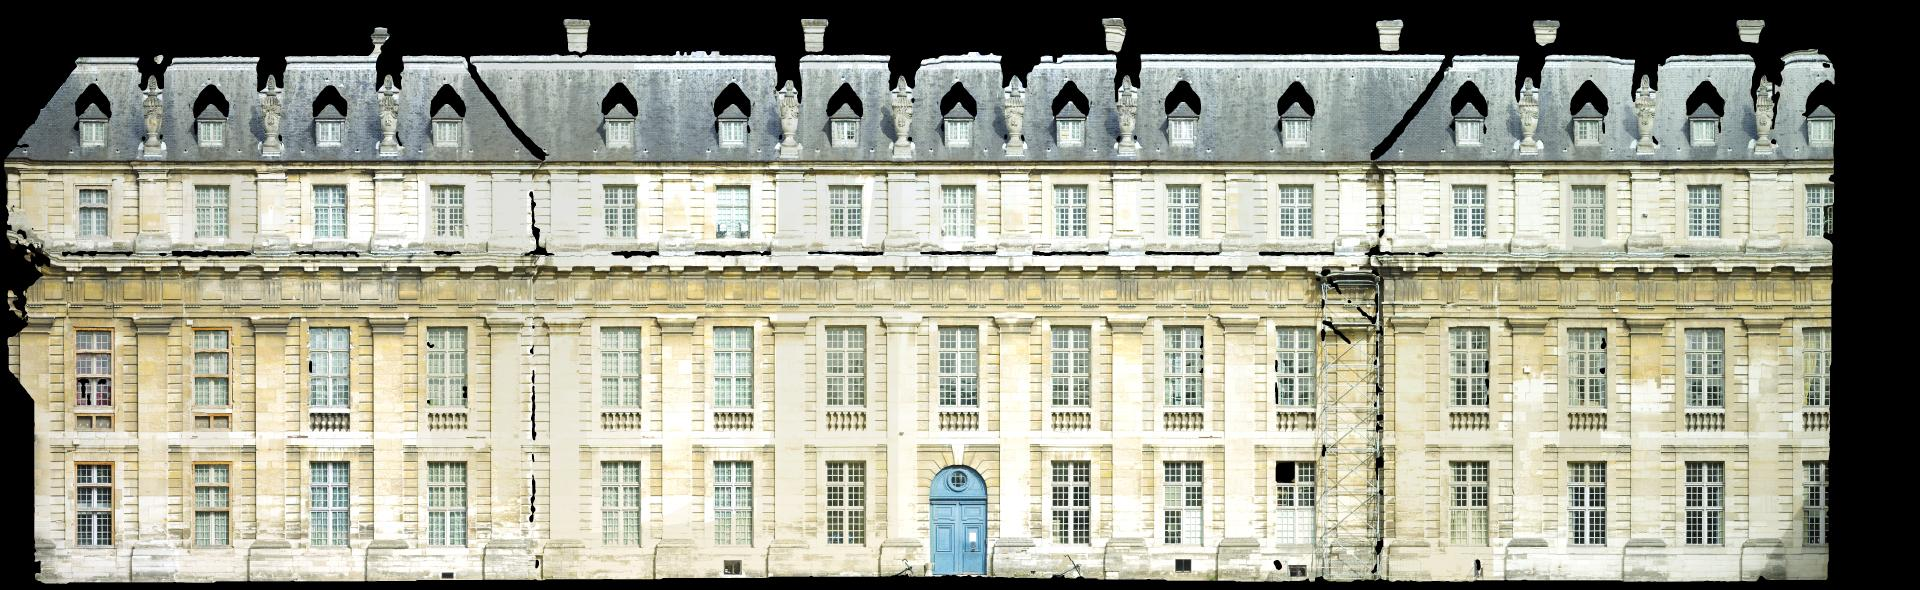
\includegraphics[width=160mm]{FIGS/Vincennes/Ortho-Eg-Test-Redr.jpg}

\end{center}
\caption{1-Depth map in ortho cylindric geometry, 2-The same, anamorphosed in euclidean
geometry, 3-Ortho photo in euclidean geometry}
\label{FIG:OK:Vincenne}
\end{figure}


Although all the tool described in this section are rather optimized 
for ortho-photo generation, it is still possible to generate 3D cloud points.
As usual in ground geometry, we use the result of matching for the 3D and
the ortho-photo for textures.
For example :


\begin{verbatim}
Nuage2Ply Malt-OC-F1/NuageImProf_Malt-Ortho-UnAnam_Etape_1.xml \
      Attr=Ortho-UnAnam-Malt-OC-F1/Ortho-Eg-Test-Redr.tif Scale=3

Nuage2Ply Malt-OC-F2/NuageImProf_Malt-Ortho-UnAnam_Etape_1.xml \
      Attr=Ortho-UnAnam-Malt-OC-F2/Ortho-Eg-Test-Redr.tif Scale=3
\end{verbatim}

The meta data file {\tt NuageImProf\_Malt-Ortho-UnAnam\_Etape\_1.xml} contains
all the information relative to the local repair use for computation  (inside
the {\tt <RepereGlob>} balise):

\begin{verbatim}
<?xml version="1.0" ?>
<XML_ParamNuage3DMaille>
     <NbPixel>5972 1834</NbPixel>
     <PN3M_Nuage>
..
     </PN3M_Nuage>
     <RepereGlob>
          <Ori>-0.00573682224569793675 -2.71135741550217935 -0.452115668474152133</Ori>
          <Ox>0.000296255688442622397 0.999999887087029138 -0.000371562236912849938</Ox>
          <Oy>-0.000437158066873386052 0.000371691728275074906 0.999999835369028367</Oy>
          <Oz>0.999999860562685972 -0.000296093208240548543 0.000437268133301418503</Oz>
     </RepereGlob>
...
  <Orientation>
....
  </Orientation>
...
</XML_ParamNuage3DMaille>
\end{verbatim}

The point cloud are then generated  in the same global repair and are
naturally mergeable as can be seen on figure~\ref{FIG:TroidD:Vincenne}.


\begin{figure}
\begin{center}
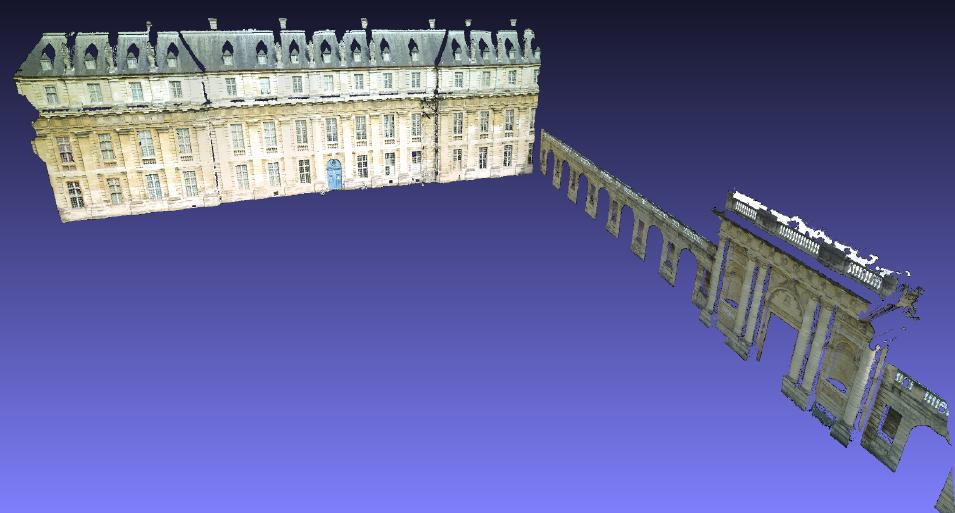
\includegraphics[width=160mm]{FIGS/Vincennes/Vinc3D.jpg}
\end{center}
\caption{Snapshot of two point clouds of the facade}
\label{FIG:TroidD:Vincenne}
\end{figure}

%-------------------------------------------------------------------
%-------------------------------------------------------------------
%-------------------------------------------------------------------






